\section{Benchmarks and Evaluation}\label{sec:benchmarks}

\paragraph{Foundational datasets.} Tufano et al.\ automated two review activities, implementing a reviewer's comment in up to 31\% of cases~\cite{tufano2021towards}. CodeReviewer defined the three tasks later reused (quality estimation, comment generation, refinement) on 1,161 GitHub repositories in nine languages, with baselines of QE F1 71.53, comment-generation BLEU-4 5.32 and refinement BLEU 82.61~\cite{li2022automating}. These datasets fixed diff-only inputs, a single reference per change and text-similarity scoring.

\paragraph{Text similarity fails.} Against human relevance judgements, BLEU reaches Kendall $\tau=0.001$ and chrF++ $\tau=0.1555$, whereas reference-free CRScore reaches $\tau=0.4567$~\cite{naik2025crscore}. A ``copy the input'' baseline scores refinement BLEU 58.75 with 0\% exact match~\cite{li2022automating}. DeepCRCEval found that a BLEU-optimised CodeReviewer scored 1.77 on actionability (1--10 scale), against about 9.4--10 for a few-shot GPT-4 reviewer~\cite{lu2025deepcrceval}.

\paragraph{Noisy ground truth.} TooNoisy found 36\% noisy comments in a 270-comment training sample~\cite{liu2025toonoisy}, and DeepCRCEval judged only 3\% (Tufano) and 8\% (CodeReviewer) of sampled references ``ideal''~\cite{lu2025deepcrceval}. Noise also runs the other way: expert verification added 1,114 issues to 391 original PR comments (+285\%) in AACR-Bench, so a model finding a real but uncommented issue is scored as a false positive~\cite{zhang2026aacr}.

\paragraph{PR-level benchmarks, low scores.} The 2025--2026 benchmarks use hundreds of verified PRs with repository context and score issue detection (Fig.~\ref{fig:benchmarks}b). Best results are modest: F1 19.38\% on SWR-Bench, rising to 21.91\% with ten aggregated runs~\cite{zeng2025swr}; F1 16.12\% on AACR-Bench, where the highest recall of 47.24\% came at 6.70\% precision~\cite{zhang2026aacr}; 15--31\% of human-flagged issues detected on SWE-PRBench~\cite{kumar2026swe}; about 33\% known-defect detection rate on CR-Bench-v2~\cite{pereira2026crbenchv2}; and a 32.1\% test pass rate for Claude Code on c-CRAB~\cite{zhang2026ccrab}. Most of these are unreviewed arXiv preprints. Synthetic data overstates capability (Fig.~\ref{fig:benchmarks}a): one study reports F1 0.847 on mutation-injected samples against 0.066 on real PRs~\cite{kumar2026bigger}, and a 7B model fell from 68.26\% F1 on BigVul to 3.09\% on PrimeVul~\cite{ding2025vulnerability}.

\paragraph{Unvalidated, incomparable judges.} LLM-as-judge is now the de facto scorer, but validation is thin and judges differ across benchmarks. SWR-Bench validated its judge on 100 reports~\cite{zeng2025swr}, SWE-PRBench reports $\kappa=0.75$ against humans~\cite{kumar2026swe}, and AACR-Bench uses a different judge model~\cite{zhang2026aacr}. No leaderboard runs the same models across benchmarks, so metrics and rankings are not comparable.

\begin{figure}[t]
\centering
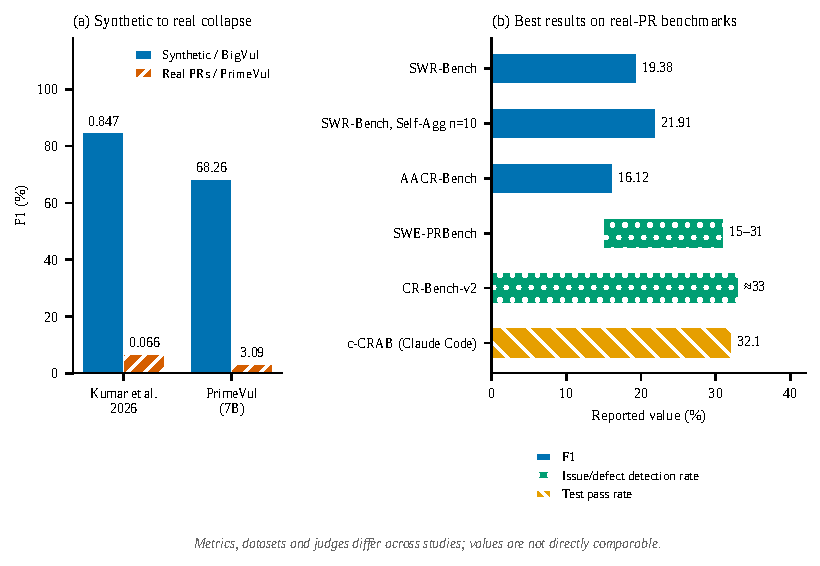
\includegraphics[width=\textwidth]{figures/benchmarks.pdf}
\caption{(a) Collapse from synthetic to real data: F1 0.847 on mutation-injected samples versus 0.066 on real PRs~\cite{kumar2026bigger}, and 7B-model F1 of 68.26\% on BigVul versus 3.09\% on PrimeVul~\cite{ding2025vulnerability}. (b) Best reported results on real-PR benchmarks, each bar labelled with its own metric: SWR-Bench F1 19.38\% (21.91\% with Self-Agg, $n=10$), AACR-Bench F1 16.12\%, SWE-PRBench 15--31\% of issues detected (interval), CR-Bench-v2 about 33\% known-defect detection, and c-CRAB 32.1\% test pass rate (Claude Code). Metrics differ and are not comparable.}
\label{fig:benchmarks}
\end{figure}
